% Informe Final -- Proyecto Final de Ingeniería Electrónica, UTN FRLR.
% Estructura según el Reglamento de Proyecto Final (sección 3).
% Compilar con `make` (Tectonic).
\documentclass[a4paper,11pt,oneside]{report}
% PROVISORIO. Reemplazar por la copia de ~/mi-preamble-latex/mypreamble.tex
% (no está en esta máquina). Se versiona acá para que el informe compile sin
% depender de rutas absolutas del home.
\usepackage{fontspec}
\usepackage[spanish, es-noshorthands]{babel}
\usepackage[a4paper, margin=25mm]{geometry}
\usepackage{microtype}

\usepackage{estilo-informe}

\newcommand{\titulotrabajo}{Decodificador MPEG-2 en MPSoC FPGA con Linux}
\newcommand{\autor}{Esteban Adriel Bustamante}
\newcommand{\tutor}{Ing.~Ricardo Maldonado}

\begin{document}
\pagenumbering{roman}
% Tapa diseñada en Scribus (tapa-scribus.pdf: contratapa, lomo y tapa en una
% sola hoja para la encuadernación). Acá se usa solo la tapa: el panel
% derecho, desde x = 596,5 pt, recortado 8 pt por lado para que mida lo mismo
% que una A4 (595 pt) sin deformarse.
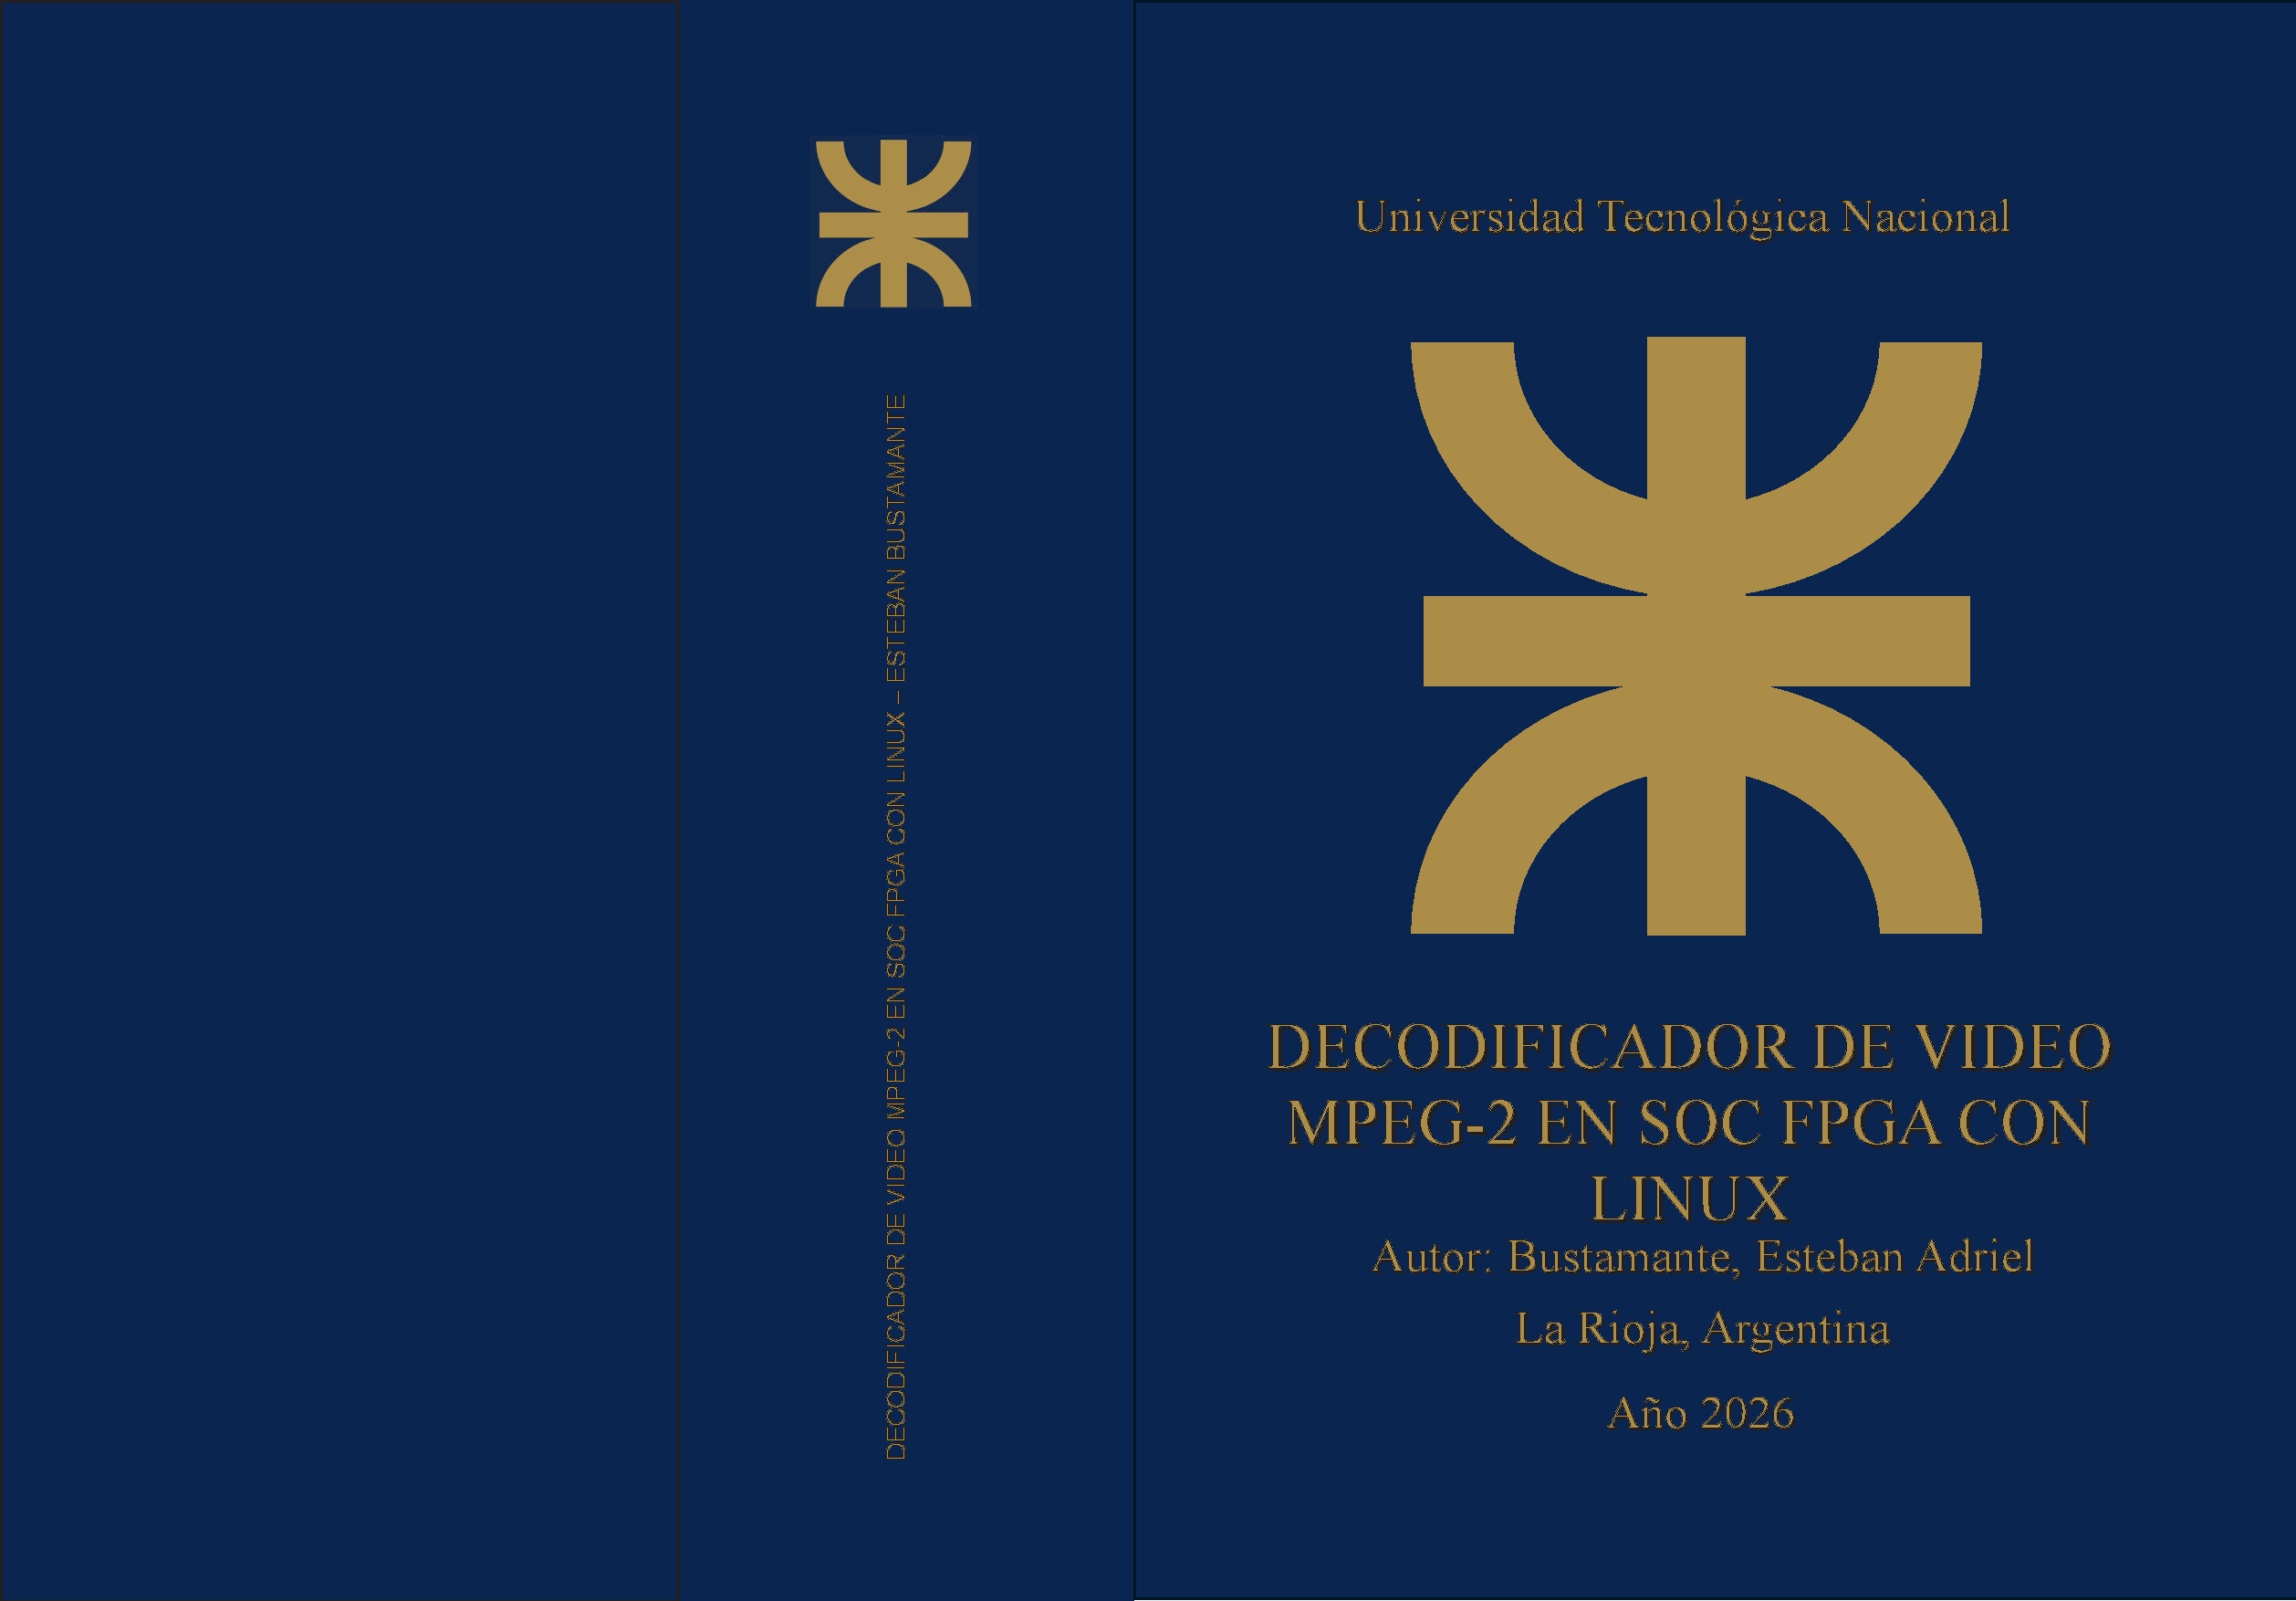
\includepdf[pages=1, viewport=604.5 0 1199.5 841.89, clip]{portada/tapa-scribus.pdf}

% Portada interior, con el contenido mínimo del modelo del Anexo 5 del
% Reglamento (cátedra, docentes, tutor, fecha de examen) que la tapa no lleva.
\begin{titlepage}
  \centering\sffamily
  {\color{m2grey} La Rioja, \fechaentrega\par}
  \vspace{2cm}
  {\Large Universidad Tecnológica Nacional --- Facultad Regional La Rioja\par}
  {\large Carrera de Ingeniería Electrónica --- Cátedra de Proyecto Final\par}
  \vspace{1cm}
  Prof.\ Ing.~Pedro Chahín Rearte \quad JTP Ing.~Oscar Almonacid\par
  \vspace{3cm}
  {\color{m2grey}Trabajo Final de Grado}\par
  {\Huge\bfseries\color{m2navy}\titulotrabajo\par}
  \vspace{4mm}{\Large\color{m2teal}\subtitulotrabajo\par}
  {\color{m2amber}\rule{0.6\textwidth}{1.4pt}\par}
  \vspace{2cm}
  {\large Autor: \autor\par}
  {\large Docente Tutor: \tutor\par}
  \vfill
  Fecha de examen: \rule{3cm}{0.4pt}
\end{titlepage}

\chapter*{Agradecimientos}
\addcontentsline{toc}{chapter}{Agradecimientos}

Al tutor, Ing.~Ricardo Maldonado, por su guía sincera y entusiasta en el
proyecto, desde la idea hasta la implementación.

A la cátedra de Proyecto Final, particularmente al Ing.~Pedro Chahín Rearte,
por su constante apoyo e interés en el proyecto, además de haberme presentado
el tema en sus magistrales clases de Electrónica Aplicada III.

A mi esposa Lucía, sin quien nada de esto hubiese sido posible, por su
incesante apoyo e instancia a no cesar en el esfuerzo de terminar este
proyecto. Sus palabras de aliento y sus muestras de cariño fueron siempre un
combustible sin el cual este trabajo no hubiese salido a flote.

A mi familia, con especial mención a Viviana, Arelisa, Lourdes y Samuel como
excepcionales técnicos de laboratorio.

A mis padres, que como dijo Kant sobre el espacio y el tiempo, han sido en mi
vida estructuras innatas (anteriores a cualquier experiencia) que han
funcionado como un «filtro» o «marco» obligatorio. No podría percibir nada si
no es a través de ellos.

A mis profesores universitarios y escolares, respectivamente José Sanguedolce
y Matías Sevilla, quienes siempre despertaron en mí el interés de compartir y
expandir los aprendizajes que esta vida me ha regalado.

A Koen De Vleeschauwer, autor de mpeg2fpga, por publicar su trabajo con
licencia libre y documentarlo tan bien.

A las comunidades de software y hardware libre cuyas herramientas hicieron
posible el proyecto (capítulo~\ref{cap:metodologia}).

\vfill
\begin{center}
  \begin{minipage}{0.78\linewidth}
    \itshape\small
    Iamque opus exegi, quod nec Iovis ira nec ignis\\
    nec poterit ferrum nec edax abolere vetustas.\\
    Cum volet, illa dies, quae nil nisi corporis huius\\
    ius habet, incerti spatium mihi finiat aevi.

    \smallskip
    \upshape\raggedleft --- Ovidio, \emph{Metamorfosis}, XV, 871--874
  \end{minipage}
\end{center}
\vfill

\begin{flushright}
  \itshape \autor\\
  La Rioja, \fechaentrega
\end{flushright}

\chapter*{Resumen}
\addcontentsline{toc}{chapter}{Resumen}

\pendiente{Media página: problema, qué se hizo (port del núcleo mpeg2fpga a
PolarFire SoC, Linux, driver, protocolo, producto), resultados clave
(bit-exactitud contra simulación, conformidad, cuadros por segundo, demo
pública) y el enfoque de producto de propiedad intelectual mayoritariamente
libre. Palabras clave.}

\tableofcontents
\listoffigures
\listoftables
\chapter*{Símbolos y convenciones}
\addcontentsline{toc}{chapter}{Símbolos y convenciones}
\begin{description}[style=nextline, leftmargin=7em, labelwidth=6em]
  \item[APB] \emph{Advanced Peripheral Bus}.
  \item[AXI] \emph{Advanced eXtensible Interface}.
  \item[CCC] \emph{Clock Conditioning Circuit} (PLL de PolarFire).
  \item[DMA] \emph{Direct Memory Access}.
  \item[FIC] \emph{Fabric Interface Controller}.
  \item[IDCT] Transformada discreta del coseno inversa.
  \item[MAD] Error absoluto medio (\emph{Mean Absolute Difference}).
  \item[MSS] \emph{Microprocessor Subsystem} del PolarFire SoC.
  \item[VLD] Decodificación de longitud variable.
\end{description}
\pendiente{Completar a medida que se redactan los capítulos.}


\cleardoublepage
\pagenumbering{arabic}
\chapter{Introducción}
\label{cap:introduccion}

% Fuentes: anteproyecto/diagnostico, anteproyecto/justificacion.
\section{Contexto y problema}
\pendiente{Diagnóstico del anteproyecto condensado: decodificación MPEG-2
en hardware, por qué FPGA, por qué un SoC con procesador.}

\section{Enfoque: el desarrollo de un producto de propiedad intelectual}
\pendiente{Idea central de la tesis: mostrar de forma pedagógica el flujo
completo --- desarrollo técnico, licencias, producción, distribución y
entregables --- con herramientas mayoritariamente libres. Vincular con el
punto 1.2 del Reglamento (aspectos técnicos, económico-financieros, legales
y de mercado).}

\section{Justificación}
\pendiente{Impacto esperado (de anteproyecto/justificacion).}

\section{Organización del documento}
\pendiente{Un párrafo por capítulo; mencionar los documentos complementarios
(guía de usuario, nota de aplicación, documentación Doxygen).}

\chapter{Objetivos y alcance}

\section{Objetivo general}
\pendiente{Reformular sobre el aprobado; corregir la norma: MPEG-2 Video es
ISO/IEC 13818-2 (el anteproyecto citaba ISO/IEC 23002-1, que es la de
precisión de la IDCT).}

\section{Objetivos específicos}
\pendiente{Lista del anteproyecto, marcando cuáles se redefinieron.}

\section{Redefinición del alcance}
\label{sec:redefinicion-alcance}
% Reglamento 2.3: se admiten las acciones "que la experiencia adquirida
% indique como oportunas y necesarias". Criterio de evaluación 3.6 (e).
\subsection{Sistema operativo: Linux en lugar de un RTOS propio}
\pendiente{Acuerdo verbal con el tutor, Ing.~Ricardo Maldonado, a comienzos
de 2026 (febrero): acotar el alcance para lograr un plazo de finalización
realista. Qué objetivos del anteproyecto reemplaza (``Diseñar el sistema
operativo'', ``Implementar el sistema operativo'', etapas 6 y 7) y a qué se
destinó ese esfuerzo (driver de kernel, protocolo, producto). La
justificación técnica va en el capítulo~\ref{cap:firmware}.}

\subsection{Salida de video}
\pendiente{La PolarFire SoC Discovery Kit no tiene conector de video: la
cadena RTL de visualización (yuv2rgb, syncgen) queda instanciada pero sin
verificar, y la conversión YUV$\to$RGB se hace en el cliente.}

\section{Alcance final}
\pendiente{Qué entra y qué no (p.\,ej.\ matrices de cuantización cargadas
como limitación conocida, si sigue abierta al entregar).}

\chapter{Marco teórico y antecedentes}
\label{cap:marco}

Este capítulo reúne lo necesario para seguir el resto del informe: cómo
comprime video MPEG-2, qué define la norma, cómo se organiza un
decodificador en hardware, cómo es el núcleo del que se partió y la
plataforma sobre la que se implementó. Cubre los objetivos de investigación
del Anteproyecto (sección~\ref{sec:obj-especificos-aprobados}).

\section{Compresión de video y la familia MPEG}

Un video sin comprimir es enorme: en definición estándar europea, $720
\times 576$ píxeles a 25 imágenes por segundo con submuestreo de color 4:2:0,
son unos 124~Mbit/s. Un flujo MPEG-2 de calidad de televisión ocupa entre 4 y
8~Mbit/s, de 15 a 30 veces menos. La compresión aprovecha cuatro tipos de
redundancia \citep{Watkinson_2013}:

\begin{itemize}
  \item \textbf{Espacial}: los píxeles vecinos se parecen. Una transformada,
    la DCT, concentra la energía de cada bloque en pocos coeficientes.
  \item \textbf{Temporal}: imágenes consecutivas se parecen. Se transmite la
    diferencia contra una predicción construida desplazando bloques de
    imágenes ya decodificadas según vectores de movimiento.
  \item \textbf{Perceptual}: el ojo es poco sensible a los detalles finos y al
    color. Los coeficientes de alta frecuencia se cuantizan con menos
    precisión, y la crominancia se submuestrea.
  \item \textbf{Estadística}: algunos valores son mucho más frecuentes que
    otros. Se codifican con códigos de longitud variable, más cortos para lo
    más frecuente.
\end{itemize}

El grupo MPEG (\emph{Moving Picture Experts Group}) de ISO e IEC estandarizó
esta combinación en sucesivas generaciones. MPEG-1 (ISO/IEC 11172) apuntó al
video en CD. MPEG-2 (ISO/IEC 13818), publicado a mediados de la década de
1990, agregó el video entrelazado y velocidades mayores, y se convirtió en el
formato de la televisión digital y del DVD. Las generaciones siguientes,
MPEG-4 Parte 2, H.264/AVC y HEVC, mantuvieron el mismo esquema híbrido
(transformada más compensación de movimiento) con herramientas más
eficientes y mucho más complejas.

\section{La norma ISO/IEC 13818}
\label{sec:norma}

La norma tiene varias partes. Las relevantes para este trabajo son la parte~1
(sistemas: cómo se multiplexan video y audio en flujos de programa y de
transporte), la parte~2 (video, \citealp{ISO_13818_2}) y la parte~4
(pruebas de conformidad, que provee los flujos de prueba usados en el
capítulo~\ref{cap:resultados}). El decodificador de este proyecto trabaja
sobre el \emph{flujo elemental} de video de la parte~2; separarlo de un flujo
de transporte o de programa queda a cargo del cliente.

\subsection{Estructura del flujo}

Un flujo de video MPEG-2 es jerárquico:

\begin{description}[style=nextline, leftmargin=1.5em]
  \item[Secuencia] Define el tamaño de imagen, la tasa de imágenes y,
    opcionalmente, matrices de cuantización propias.
  \item[Grupo de imágenes (GOP)] Un conjunto de imágenes que empieza en una
    imagen decodificable por sí sola.
  \item[Imagen] De tres tipos. Las \textbf{I} se codifican sin referencia a
    otras. Las \textbf{P} se predicen desde la imagen I o P anterior. Las
    \textbf{B} se predicen desde una anterior y una posterior, por lo que el
    orden del flujo no coincide con el de presentación: el decodificador
    debe reordenar.
  \item[Rebanada (\emph{slice})] Una franja de macrobloques que permite
    resincronizar ante errores.
  \item[Macrobloque] $16 \times 16$ píxeles de luminancia: en 4:2:0, cuatro
    bloques de luminancia y dos de crominancia de $8 \times 8$, que comparten
    vectores de movimiento.
  \item[Bloque] $8 \times 8$ coeficientes de la DCT.
\end{description}

\subsection{Perfiles y niveles}

La norma agrupa herramientas en \emph{perfiles} y límites de tamaño y
velocidad en \emph{niveles}. El más difundido es el Main Profile en Main
Level (MP@ML): imágenes de hasta $720 \times 576$, hasta 30 imágenes por
segundo y hasta 15~Mbit/s, que cubre la televisión de definición estándar y
el DVD. El High Level extiende los límites a la alta definición.

\subsection{El proceso de decodificación}
\label{sec:proceso-decodificacion}

Para cada bloque, el decodificador:

\begin{enumerate}
  \item \textbf{Decodifica los códigos de longitud variable}, que dan pares
    de \emph{corrida} (cantidad de ceros) y \emph{nivel} (valor del
    coeficiente siguiente), además de los vectores de movimiento y las
    cabeceras.
  \item \textbf{Expande las corridas} y \textbf{reordena} los coeficientes
    del recorrido en zigzag (o alternado, para video entrelazado) a la
    matriz de $8 \times 8$.
  \item \textbf{Cuantiza inversamente}: multiplica cada coeficiente por un
    factor de escala y por el elemento correspondiente de una matriz de
    cuantización. Hay matrices por defecto, distintas para bloques intra y
    no intra, y la secuencia puede reemplazarlas por matrices propias. Este
    detalle importa: el error de conformidad que quedó abierto en este
    proyecto está en el camino de carga de esas matrices.
  \item \textbf{Aplica la IDCT}, que devuelve el bloque al dominio de los
    píxeles. La norma no fija una implementación exacta, sino una precisión
    mínima, definida originalmente por el estándar IEEE~1180-1990
    \citep{IEEE_1180_1990} y hoy por ISO/IEC 23002-1. Dos decodificadores
    conformes pueden diferir en una unidad en algunos píxeles.
  \item \textbf{Compensa el movimiento}: en las imágenes P y B, suma al
    resultado la predicción leída de las imágenes de referencia, desplazada
    con precisión de medio píxel.
\end{enumerate}

Las imágenes reconstruidas se guardan en una memoria de cuadros, porque las
I y P son referencia de las siguientes, y se entregan en orden de
presentación.

\section{Decodificación de video en hardware}
\label{sec:arquitecturas-vlsi}

Un procesador moderno decodifica MPEG-2 por software sin dificultad. Las
implementaciones en hardware se justifican cuando importan el consumo, el
costo por unidad o el comportamiento determinista: receptores de televisión,
reproductores, equipos embebidos. Sus arquitecturas comparten algunos rasgos
\citep{Watkinson_2013}:

\begin{itemize}
  \item \textbf{Tubería de función fija}: cada etapa del
    proceso de la sección~\ref{sec:proceso-decodificacion} es un bloque de
    hardware dedicado, y los bloques trabajan en paralelo sobre datos
    sucesivos, a razón de un coeficiente o un píxel por ciclo.
  \item \textbf{FIFOs entre etapas}: absorben las diferencias de ritmo entre
    etapas cuya carga varía según el contenido.
  \item \textbf{Memoria externa}: la memoria de cuadros no cabe en el chip.
    El ancho de banda hacia ella, compartido por la escritura de imágenes,
    la lectura de referencias para la compensación de movimiento y la lectura
    para visualización, suele ser el recurso más disputado.
  \item \textbf{Varios dominios de reloj}: la decodificación, la memoria y
    la salida de video corren a frecuencias distintas.
\end{itemize}

\section{El núcleo mpeg2fpga}
\label{sec:mpeg2fpga}

mpeg2fpga es un decodificador MPEG-2 en Verilog escrito por Koenraad De
Vleeschauwer entre 2007 y 2009 y publicado en OpenCores en 2017 con licencia
BSD \citep{De_Vleeschauwer_2017}. Decodifica flujos elementales MP@ML (y,
con otra configuración del mapa de memoria, de alta definición), con
submuestreo 4:2:0, y fue desarrollado y probado sobre una placa Xilinx ML505
con una FPGA Virtex-5. Su documentación \citep{De_Vleeschauwer_2009_guide}
es detallada y fue la referencia principal de este trabajo.

\begin{figure}[ht]
  \centering
  \begin{tikzpicture}[
      e/.style={blk, minimum width=24mm, minimum height=10mm, font=\sffamily\scriptsize},
      ed/.style={e, draw=m2grey, fill=m2grey!8},
      node distance=9mm and 5mm]
    \node[e] (in) {Entrada del\\flujo};
    \node[e, right=of in] (vbuf) {Buffer de\\video};
    \node[e, right=of vbuf] (gb) {Getbits};
    \node[e, right=of gb] (vld) {VLD};
    \node[e, below=of vld] (rld) {Corridas, cuant.\\inversa, zigzag};
    \node[e, left=of rld] (idct) {IDCT};
    \node[e, left=of idct] (mc) {Compensación\\de movimiento};
    \node[e, left=of mc] (fs) {Memoria de\\cuadros};
    \node[ed, below=of fs] (res) {Remuestreo\\de croma};
    \node[ed, right=of res] (mix) {Mezcla\\y OSD};
    \node[ed, right=of mix] (rgb) {YUV a RGB};
    \node[ed, right=of rgb] (out) {Salida de\\video};
    \node[e, left=8mm of fs, draw=m2teal, fill=m2teal!8] (mem) {Memoria\\externa};
    \draw[arr] (in) -- (vbuf); \draw[arr] (vbuf) -- (gb); \draw[arr] (gb) -- (vld);
    \draw[arr] (vld) -- (rld); \draw[arr] (rld) -- (idct); \draw[arr] (idct) -- (mc);
    \draw[arr] (mc) -- (fs); \draw[arr] (fs) -- (res);
    \draw[arr] (res) -- (mix); \draw[arr] (mix) -- (rgb); \draw[arr] (rgb) -- (out);
    \draw[arr] (vld.south west) -- node[lbl, fill=white, inner sep=1pt, pos=0.5] {vectores} (mc.north east);
    \draw[arr, <->] (mem) -- (fs);
  \end{tikzpicture}
  \caption{Tubería del núcleo mpeg2fpga, adaptada de
    \citet{De_Vleeschauwer_2009_guide}. En gris, la cadena de visualización,
    que en este proyecto no tiene salida física.}
  \label{fig:tuberia}
\end{figure}

\paragraph{Tubería}
La figura~\ref{fig:tuberia} muestra sus etapas. El flujo entra a un buffer
de video, que en realidad vive en la memoria externa y actúa como una gran
FIFO elástica entre la tasa de llegada y la de decodificación. \emph{Getbits}
ofrece una ventana deslizante sobre el flujo para que el VLD extraiga códigos
de longitud variable. Los coeficientes pasan por la decodificación de
corridas, la cuantización inversa y la IDCT; el error de predicción
resultante se suma a la predicción que arma la compensación de movimiento, y
la imagen reconstruida se escribe en la memoria de cuadros. En paralelo, la
cadena de visualización lee las imágenes terminadas y genera la señal de
video.

\paragraph{Interfaces}
El núcleo se comunica con el exterior por cuatro interfaces: la entrada del
flujo (un byte por ciclo con control de flujo), un banco de registros para el
procesador que lo controla, un puerto de memoria externa y la salida de
video. Todo el acceso a memoria pasa por un único árbitro que etiqueta cada
lectura para devolver la respuesta al cliente correcto. El mapa de memoria
por defecto necesita 4~MB, y la variante de alta definición, 16~MB.

\paragraph{Control}
El banco de registros expone las propiedades del flujo (tamaño, tasa de
imágenes, estado), habilita interrupciones y controla los modos de
reproducción especiales: pausa, repetición de imagen y cambio de flujo sin
\emph{reset}. Un \emph{watchdog} reinicia el decodificador si deja de
progresar mientras tiene trabajo pendiente.

\paragraph{Dependencias de Xilinx}
Las FIFOs y memorias se definen en un archivo de envoltorios que puede usar
primitivas de Virtex-5 o implementaciones portables, y los tres relojes
llegaban desde afuera. El controlador de memoria era el de la placa ML505.
Estas dependencias son las que el port tuvo que resolver
(sección~\ref{sec:port}).

\section{PolarFire SoC}
\label{sec:polarfire}

PolarFire SoC es una familia de Microchip que integra en un chip un tejido
FPGA y un subsistema de microprocesadores RISC-V
\citep{Microchip_MSS_TRM}. A diferencia de las FPGA basadas en SRAM, su
configuración se guarda en celdas no volátiles: el chip arranca configurado
y su consumo estático es bajo.

\paragraph{El subsistema de microprocesadores (MSS)}
Tiene cinco núcleos RISC-V de 64 bits: un E51 de monitoreo, que ejecuta el
firmware de arranque, y cuatro U54 de aplicación (RV64GC, con unidad de
punto flotante y gestión de memoria), capaces de correr Linux. Los acompañan
un subsistema de memoria L2 compartido, un controlador de memoria DDR,
controladores de periféricos (Ethernet, USB, tarjeta SD, UART) y un
controlador de interrupciones. Los controladores de interfaz con el tejido
(FIC) lo comunican con la lógica de la FPGA en ambos sentidos, por buses
AXI4 y APB.

Un detalle de la L2 resultó importante durante el desarrollo: es una caché
\emph{del lado de la memoria}, seleccionada por la ventana de direcciones con
que se accede a la DDR, no por los atributos de las páginas. Esto hizo que
dos ventanas que en realidad mostraban la misma memoria parecieran
independientes en las pruebas (sección~\ref{sec:problemas}).

\paragraph{La placa}
La PolarFire SoC Discovery Kit \citep{Microchip_Discovery_UG} es una placa de
bajo costo con el dispositivo MPFS095T (unas 95\,000 celdas lógicas), memoria
DDR4, Ethernet, ranura microSD y un programador JTAG integrado accesible por
USB. No tiene salida de video ni monitores de consumo, dos limitaciones que
condicionaron el alcance (secciones~\ref{sec:redef-video}
y~\ref{sec:modelo-potencia}).

\section{Antecedentes}
\label{sec:antecedentes}

La decodificación de MPEG-2 en hardware es un problema maduro, resuelto
industrialmente en circuitos integrados de receptores y reproductores desde
la década de 1990. En el ámbito académico y abierto, los antecedentes
relevantes para este trabajo son:

\begin{itemize}
  \item \textbf{El propio mpeg2fpga} \citep{De_Vleeschauwer_2017}, que
    demostró un decodificador completo en una FPGA, con su banco de
    simulación y sus pruebas de conformidad. Es la base tecnológica del
    proyecto.
  \item \textbf{Arquitecturas mixtas procesador--FPGA}, como la de
    \citet{Billaud_2004}, que aborda la implementación de un decodificador
    MPEG-2 repartiendo el trabajo entre un procesador y lógica
    programable: el mismo tipo de partición que este proyecto lleva a un SoC
    con ambos en un mismo chip.
  \item \textbf{Decodificadores de software}, como el de referencia del MPEG
    Software Simulation Group, usado aquí para verificar la corrección.
\end{itemize}

No se encontró un trabajo publicado que lleve mpeg2fpga a PolarFire SoC ni,
en general, un decodificador MPEG-2 abierto integrado con Linux en un SoC FPGA
con procesadores RISC-V, documentado como producto. Ese es el aporte de este
trabajo: no un algoritmo nuevo, sino el recorrido completo, verificado y
reproducible, desde un núcleo abierto hasta un producto distribuible.

\chapter{Metodología y flujo de desarrollo}

\section{Flujo de desarrollo de un producto de IP}
\pendiente{Diagrama del flujo completo: investigación $\to$ port $\to$
integración $\to$ bring-up $\to$ firmware $\to$ verificación $\to$ release.}
\section{Organización del repositorio y control de versiones}
\pendiente{Ramas por tipo de contenido (docs, hardware, firmware), worktrees.}
\section{Verificación}
\pendiente{Simulación primero (Icarus), bancos unitarios (IEEE 1180), TDD y
KUnit en el driver, harness de regresión, comparación de cuadros.}
\section{Bitácoras de bring-up}
\pendiente{Las notas numeradas de docs/bringup como cuaderno de ingeniería;
lección: un testbench verde solo prueba la propia hipótesis.}
\section{Herramientas utilizadas}
\label{sec:herramientas}
\pendiente{Gráfico de todas las herramientas libres usadas, cuáles fueron
prioritarias y una descripción corta de su uso; contraste con las
propietarias inevitables (Libero SoC). Tabla completa en el
anexo~\ref{anx:herramientas}.}

\chapter{Desarrollo de hardware}

\label{cap:hardware}
\section{Arquitectura del sistema}
\pendiente{Diagrama de bloques: MSS, FIC, puentes, núcleo, DDR.}
\section{Port del núcleo a PolarFire}
\pendiente{FIFOs blandos (xfifo\_sc/xfifo\_dc), CCC, clocks.}
\section{Integración con el MSS}
\pendiente{Puente APB (registros), mem2axi\_bridge, stream DMA, interrupción
de imagen, build id.}
\section{Problemas de integración relevantes}
\pendiente{Selección pedagógica: extensión de signo del parámetro, alias de
udmabuf y L2, puertos compartidos de la RAM del FIFO (uram), PSTRB, PLL
apagado.}
\section{Optimización del rendimiento}
\pendiente{Pipelining del puente de memoria (7{,}2 $\to$ 22--23 fps),
localización del cuello de botella en motcomp\_recon.}

\chapter{Desarrollo de firmware}

\label{cap:firmware}
\section{Linux en el MSS}
\pendiente{Por qué Linux (ver sección~\ref{sec:redefinicion-alcance}):
drivers, red y TLS disponibles; esfuerzo volcado al producto.}
\section{Driver de kernel}
\pendiente{Mapa de registros, sysfs, dispositivo misc y eventos, overlays,
KUnit.}
\section{Daemon y protocolo v1}
\pendiente{Contrato de red, seguridad (token, TLS opcional), streaming con
control de flujo.}
\section{Biblioteca cliente en Python}
\pendiente{}
\section{Demostración en vivo}
\pendiente{Relay público, transporte H.264/MediaSource, capturas de
figuras/demo\_web.}

\chapter{El producto: propiedad intelectual, producción y distribución}

\section{Licencias de los componentes}
\pendiente{Núcleo mpeg2fpga (tipo BSD), Linux y driver (GPL) y oferta de
código fuente, herramientas propietarias (Libero SoC), contenido de prueba
(Tears of Steel, CC-BY 3.0). Qué puede quedar cerrado (bitstream) y qué no.}
\section{Patentes de MPEG-2}
\pendiente{Vencimiento de las patentes del pool MPEG LA y su efecto sobre la
viabilidad del producto.}
\section{Propiedad intelectual del trabajo final}
\pendiente{Reglamento 4.1 (propiedad del autor) y 4.3 (depósito en el RIA,
cesión no exclusiva).}
\section{Producción}
\pendiente{Imagen de fábrica, programación del dispositivo.}
\section{Distribución y actualizaciones}
\pendiente{Releases versionadas, paquete de actualización firmado, CI,
calificación (release/qualify.sh).}
\section{Entregables}
\pendiente{Dispositivo programado, guía de usuario, nota de aplicación,
documentación Doxygen, notas de versión con informe de conformidad.}

\chapter{Análisis económico y de mercado}
\label{cap:economico}

El proyecto fue financiado íntegramente por el autor, sin auspiciantes ni
aportes de la Universidad. Este capítulo resume lo que costó desarrollarlo y
dónde podría ubicarse el resultado. El análisis es deliberadamente breve: la
cifra más significativa no es un monto, sino que el costo de herramientas fue
nulo.

\section{Costo de materiales}

El hardware se reduce a la placa de desarrollo y a una caja para protegerla
durante el trabajo (tabla~\ref{tab:costo-materiales}). No se fabricó ninguna
placa propia.

\begin{table}[ht]
  \centering
  \begin{tabular}{lr}
    \toprule
    \textbf{Ítem} & \textbf{Costo (USD)} \\
    \midrule
    PolarFire SoC Discovery Kit & 128 \\
    Caja estanca de protección & 5 \\
    \midrule
    \textbf{Total} & \textbf{133} \\
    \bottomrule
  \end{tabular}
  \caption{Costo de materiales del prototipo.}
  \label{tab:costo-materiales}
\end{table}

\section{Costo de herramientas y licencias}

Cero. Todas las herramientas libres del capítulo~\ref{cap:metodologia} son
gratuitas, y la única herramienta imprescindible sin alternativa libre,
Libero SoC, se usó con la licencia Silver, que Microchip otorga sin costo
para los dispositivos de menor capacidad (sección~\ref{sec:licencias}). Los
servicios de alojamiento del repositorio, de las versiones y de la
demostración pública también se usaron en sus modalidades gratuitas.

Este resultado no es un detalle: es lo que hace reproducible el proyecto.
Cualquier estudiante con una placa de USD 128 puede repetir el desarrollo
completo, desde la simulación hasta la liberación de una versión, sin pagar
una sola licencia. Un producto comercial que requiriera un dispositivo más
grande sí necesitaría una licencia paga de Libero.

\section{Esfuerzo de ingeniería}

El esfuerzo se estima en unas dos horas por día hábil durante un año, es
decir, del orden de \textbf{490 horas} de trabajo, a cargo de una sola
persona.

\section{Análisis de mercado}

\paragraph{El contexto}
MPEG-2 es un estándar maduro. Los códecs posteriores lo superan en
eficiencia de compresión, y cualquier procesador moderno lo decodifica por
software sin esfuerzo. Pero sigue presente en la televisión digital de
varios países, en el DVD, en equipos de difusión y en grandes archivos de
video. Y, desde el vencimiento de sus patentes en 2018
(sección~\ref{sec:patentes}), es el único códec de video de uso masivo que
puede implementarse en hardware sin pagar regalías en casi todo el mundo.

\paragraph{Dónde tiene sentido este producto}
No compite con los decodificadores integrados en circuitos de consumo, que
cuestan centavos a escala, ni con la decodificación por software. Su lugar
está en tres nichos:

\begin{itemize}
  \item \textbf{Formación}: una plataforma abierta, documentada y verificada
    para enseñar decodificación de video en hardware, integración de un núcleo
    de propiedad intelectual con un procesador y el ciclo completo de un
    producto. Es el uso más natural, y el que motivó el proyecto.
  \item \textbf{Sistemas embebidos con FPGA}: equipos que ya tienen una FPGA
    y necesitan decodificar MPEG-2 con consumo bajo y comportamiento
    determinista, sin agregar un procesador dedicado al video.
  \item \textbf{Base para otros desarrollos}: un diseño de referencia libre
    sobre el que portar el núcleo a otras FPGA o extenderlo, con un proceso
    de verificación y de liberación ya resuelto.
\end{itemize}

\paragraph{Modelo}
Las licencias elegidas definen el modelo: el producto es abierto, y su valor
está en el diseño verificado, la documentación y el proceso, no en el
secreto. La licencia recíproca del hardware propio
(sección~\ref{sec:licencia-propia}) asegura que ese valor siga disponible
para quien lo reutilice.

\chapter{Descripción del modelo experimental y simulado}
\label{cap:modelo}

Este capítulo describe con qué se obtuvieron los resultados del
capítulo~\ref{cap:resultados}: el modelo simulado, el montaje experimental y
los métodos de medición. Todas las herramientas son parte del repositorio y
pueden volver a ejecutarse.

\section{Modelo simulado}
\label{sec:modelo-simulado}

\paragraph{Simulación del núcleo completo}
El banco de prueba de Icarus Verilog, heredado del proyecto original y
adaptado al port, instancia el núcleo con un modelo de comportamiento de la
memoria externa, le entrega un flujo elemental MPEG-2 desde un archivo y
vuelca el contenido de la memoria de cuadros. El volcado se hizo idéntico,
palabra por palabra, al que se obtiene leyendo la DDR en la placa, de modo
que simulación y hardware se analizan con exactamente las mismas
herramientas.

\paragraph{Bancos de bloque}
Cada bloque nuevo tiene su banco propio (sección~\ref{sec:verificacion-rtl}):
puente APB, puente de memoria contra un esclavo AXI con latencias y
reordenamiento variables, DMA del flujo y ruta de respuestas de memoria con
el COREFIFO de Microchip.

\paragraph{Banco IEEE 1180}
Un banco dedicado alimenta la IDCT del núcleo, el mismo archivo Verilog que
se sintetiza, con los bloques pseudoaleatorios que define el estándar
IEEE~1180-1990 para sus seis condiciones de prueba (tres rangos de valores,
con los dos signos, 10\,000 bloques cada una) y compara la salida contra una
IDCT de referencia en doble precisión.

\section{Modelo experimental}
\label{sec:modelo-experimental}

\paragraph{Montaje}
La plataforma es una PolarFire SoC Discovery Kit (dispositivo MPFS095T,
encapsulado FCSG325), alojada en una caja estanca para protegerla durante el
desarrollo. Se conecta a una computadora de escritorio con Linux por:

\begin{itemize}
  \item USB, que en la placa da acceso a JTAG, para programar la FPGA y leer
    registros internos con SmartDebug, y a las consolas serie del MSS;
  \item Ethernet, en la misma red local, para operar la placa por SSH y para
    el protocolo de red.
\end{itemize}

La placa arranca Linux desde una tarjeta microSD. La computadora ejecuta
Libero SoC, las herramientas de verificación y el proceso de liberación.

\paragraph{Flujos de prueba}
Se usaron 39 flujos de conformidad MPEG-2 de distintos fabricantes y
laboratorios (CCETT, General Instrument, HHI, IBM, Nokia, Sony,
Tektronix, Toshiba, entre otros), con resoluciones de $32 \times 32$ a
$720 \times 576$. Para la demostración se usó un fragmento de \emph{Tears of
Steel} \citep{Blender_2012_tears}, codificado en MPEG-2 a $352 \times 288$ y
24 imágenes por segundo.

\paragraph{Referencia}
La referencia de corrección es \cmd{mpeg2decode}, el decodificador de
software del MPEG Software Simulation Group, incluido en el repositorio.

\section{Comparación de imágenes}
\label{sec:framecmp}

Saber si una imagen decodificada es correcta resultó más difícil de lo
esperado. La primera métrica daba un error absoluto medio cercano a 121 sobre
255 en imágenes que, vistas, eran correctas. La herramienta \cmd{framecmp}
resolvió las trampas que lo explicaban:

\begin{itemize}
  \item el núcleo guarda los píxeles como enteros con signo desplazados en
    $-128$, y se los estaba leyendo sin signo;
  \item en cada palabra de 64 bits, el píxel de la izquierda ocupa los bits
    más significativos, al revés que el orden de los bytes en memoria;
  \item la memoria de cuadros tiene cuatro buffers que rotan, y el orden de
    decodificación no es el de presentación: no hay una correspondencia fija
    entre buffer e imagen, así que cada buffer se compara contra todas las
    imágenes de referencia y se toma la mejor;
  \item los nombres internos de los planos de crominancia están cruzados
    respecto del estándar;
  \item un flujo cortado en cualquier byte deja una imagen parcial, y un
    volcado tomado durante la reconstrucción muestra una imagen a medio
    escribir: los flujos se cortan en frontera de imagen y el volcado espera
    a que la memoria deje de cambiar.
\end{itemize}

Para cada plano (Y, Cb, Cr) se reportan el error absoluto medio (MAD) y el
error pico, en niveles de 0 a 255. El método se validó primero en
simulación, hasta obtener cero donde debía haber cero, y recién después se
usó con el hardware.

\section{Regresión}
\label{sec:regresion}

El \emph{harness} \cmd{regress} ejecuta, desde la computadora y en unos 16
minutos, cuatro pruebas contra la placa:

\begin{description}[style=nextline, leftmargin=1.5em]
  \item[Conformidad] Cada flujo, cortado a 8 imágenes, se decodifica en la
    placa y se compara contra la referencia. Cada flujo recibe un veredicto
    según su peor buffer: \emph{bit-exacto} (MAD 0), \emph{cercano}
    (MAD $\leq 1$) o \emph{deriva} (MAD $> 1$), o \emph{sin escritura} si
    el núcleo no escribió ninguna imagen.
  \item[Determinismo] Un mismo flujo, cinco veces con \emph{reset} del
    núcleo y cinco cambiando de flujo sin \emph{reset}: todas las
    decodificaciones deben ser idénticas.
  \item[Robustez] Tres entradas dañadas (un flujo truncado, 200 bits
    invertidos en los datos y 256~KiB de bytes aleatorios), cada una seguida
    de un flujo correcto sin \emph{reset}, que debe decodificarse bit-exacto.
  \item[Velocidad] La memoria de cuadros se llena con un patrón conocido, se
    inicia el DMA y se mide el tiempo hasta la última escritura en la
    memoria de cuadros. Cinco corridas por flujo, después de una de
    calentamiento.
\end{description}

Los resultados se comparan contra una línea de base versionada, y la
comparación es insensible a la rotación de los buffers, que varía entre
corridas sin que cambie nada.

\section{Estimación de potencia}
\label{sec:modelo-potencia}

La Discovery Kit no permite medir el consumo por software: no tiene monitores
de corriente ni reguladores con interfaz digital, y sus puntos de prueba solo
sirven para medir tensión. Por eso la potencia se estimó con SmartPower, la
herramienta de Microchip, sobre la netlist ya ubicada y ruteada, en modo sin
vectores (con tasas de conmutación estimadas) y con las frecuencias reales
de cada reloj. Un script propio suma el resultado por instancia para obtener
la potencia de cada módulo del diseño.

\chapter{Resultados}
\label{cap:resultados}

\section{Equivalencia entre hardware y simulación}

El resultado más fuerte del proyecto es también el más simple de enunciar:
\textbf{el port reproduce el diseño original bit a bit}. Con el flujo
\cmd{tcela-17} decodificado completo en la placa y en la simulación del
núcleo, las dos memorias de cuadros resultaron idénticas byte a byte, en los
tres planos y en los cuatro buffers. La misma igualdad se observó en los
valores de error contra la referencia de todos los flujos comparados por
ambos caminos, idénticos hasta el tercer decimal.

Esto delimita responsabilidades (sección~\ref{sec:limites-simulacion}):
cualquier diferencia que quede contra el decodificador de referencia ya
estaba en el diseño original, y no fue introducida por el port.

\section{Precisión de la IDCT}

La IDCT del núcleo cumple las seis condiciones del estándar IEEE~1180-1990
(tabla~\ref{tab:ieee1180}), con el error pico en el máximo permitido de~1 y
los errores cuadráticos y medios uno o dos órdenes de magnitud por debajo de
sus límites.

\begin{table}[ht]
  \centering\small
  \begin{tabular}{@{}l r r r@{}}
    \toprule
    \textbf{Métrica} & \textbf{Peor caso medido} & \textbf{Límite} & \\
    \midrule
    Error pico                       & 1        & 1      & cumple \\
    Error cuadrático por posición    & 0,0052   & 0,06   & cumple \\
    Error cuadrático global          & 0,0036   & 0,02   & cumple \\
    Error medio por posición         & 0,0016   & 0,015  & cumple \\
    Error medio global               & 0,000056 & 0,0015 & cumple \\
    \bottomrule
  \end{tabular}
  \caption{IDCT contra IEEE 1180-1990: peor valor entre las seis
    condiciones.}
  \label{tab:ieee1180}
\end{table}

\section{Conformidad}
\label{sec:res-conformidad}

\paragraph{Imágenes intra}
En las imágenes codificadas sin predicción, la salida del hardware difiere
de la referencia en un MAD de 0,004 a 0,005 con error pico~1, en luma y en
crominancia, en cuatro flujos distintos. Es la única diferencia que el
estándar admite entre dos implementaciones conformes de la IDCT. Un flujo
completo, \cmd{mcp10ccett} ($720 \times 576$, con imágenes I, P y B), es
bit-exacto contra la referencia en todos sus buffers y planos.

\paragraph{Batería de conformidad}
La tabla~\ref{tab:conformidad} resume los veredictos sobre los 39 flujos;
el detalle está en el anexo~\ref{anx:regresion}.

\begin{table}[ht]
  \centering\small
  \begin{tabularx}{\linewidth}{@{}l r X@{}}
    \toprule
    \textbf{Veredicto} & \textbf{Flujos} & \textbf{Observación} \\
    \midrule
    Bit-exacto      & 3  & \cmd{mcp10ccett}, \cmd{tcela-15}, \cmd{tcela-17} \\
    Cercano         & 34 & MAD $\leq 0{,}04$ y pico $\leq 4$ en el peor buffer \\
    Deriva          & 0  & \\
    Sin escritura   & 2  & MPEG-1, que el núcleo no decodifica \\
    \bottomrule
  \end{tabularx}
  \caption{Veredictos de conformidad (39 flujos, hasta 8 imágenes cada uno).}
  \label{tab:conformidad}
\end{table}

Los 37 flujos MPEG-2 decodifican bit-exactos o cercanos, y en los cercanos
la diferencia es la que admite el estándar entre dos IDCT conformes: el
peor buffer de toda la batería tiene MAD 0,038 (\cmd{att-mismatch}, un
flujo de $32 \times 32$ hecho justamente para estresar la IDCT), y en 30 de
los 34 el peor buffer está por debajo de 0,02. Ningún flujo deriva. Para
llegar ahí hubo que corregir la referencia
(sección~\ref{sec:conformidad-referencia}), la forma de cortar los flujos y
dos errores del diseño original (sección~\ref{sec:conformidad-upstream}).

Los dos flujos MPEG-1 (\cmd{mei-16-long}, \cmd{mei-16v2}) no tienen
\emph{sequence extension}: el núcleo es solo MPEG-2, y el propio diseño
original los marca como no soportados.

\cmd{tcela-15} figuraba también como \emph{sin escritura}. Es un flujo de
prueba de relleno: cada imagen trae unos pocos cientos de bytes de datos y
después unos 60~KB de ceros. Su contenido es gris medio uniforme, que la
memoria de cuadros guarda como ceros, y la comparación consideraba
\enquote{nunca escrito} a todo buffer uniforme. Ahora un buffer se considera
vacío solo si tiene el valor con que el núcleo limpia la memoria al
arrancar o el que la captura escribe antes de cada prueba. Con ese
criterio, \cmd{tcela-15} es bit-exacto. Por el servicio de red también
entrega sus 8 imágenes completas.

\subsection{Un error en la referencia}
\label{sec:conformidad-referencia}

La primera versión de esta batería daba un resultado muy distinto: un solo
flujo bit-exacto, 12 cercanos y 23 con deriva, de los cuales once fallaban
desde la primera imagen con MAD de 12 a 18. Todos ellos cargan una matriz de
cuantización propia en la cabecera de secuencia, y casi todos cargan
literalmente la matriz por defecto, lo que debería ser equivalente a no
cargar ninguna. La conclusión natural fue un error en el camino de carga de
matrices del núcleo, y así figuró como limitación conocida.

Dos observaciones la desmintieron. La documentación del diseño original
declara aprobados todos esos flujos. Y una simulación del núcleo con un
monitor sobre la memoria de la matriz mostró que las 64 escrituras llegaban
a la dirección correcta con el valor correcto. Al mirar las imágenes en
lugar de los números, la del hardware era nítida y la de la referencia una
imagen en bloques. El error estaba en la copia de \cmd{mpeg2decode} que
acompaña al núcleo: en la cabecera de secuencia, la lectura de las matrices
había quedado dentro de un \cmd{if} que solo se ejecuta con las trazas
activadas. Sin trazas, que es como la usa la comparación, la referencia no
cargaba la matriz ni consumía sus 512~bits.

Corregido ese \cmd{if}, las capturas del hardware, idénticas byte a byte a
las anteriores, pasaron a 2 bit-exactos, 29 cercanos y 5 con deriva:
\cmd{gi4} bajó de MAD 17,9 a 0,005 en su imagen intra. La corrección también resolvió la mayor parte de la deriva en
imágenes predichas, porque varios de esos flujos cargan matrices para
bloques no intra.

\subsection{Dos errores en el diseño original}
\label{sec:conformidad-upstream}

Corregida la referencia quedaban cinco flujos con deriva. En dos de ellos
(\cmd{sony-ct1}, \cmd{hhi-burst-long}) el corte de 8 imágenes terminaba en
el primer campo de un cuadro; ahora el corte nunca separa los dos campos.
Los otros tres (\cmd{nokia6-60}, \cmd{tcela-10}, \cmd{tcela-14}) eran
errores del núcleo: la simulación del RTL original da el mismo volcado, bit
a bit, que la placa, así que no los introdujo el port, aunque la
documentación original da esos flujos por aprobados.

Simular hasta las imágenes afectadas lleva horas por volcado. El método que
funcionó fue otro: modificar una copia de la referencia para que se
comporte como se sospecha que se comporta el hardware, y ver si los
volcados de la placa coinciden con ella al nivel de ruido de la IDCT. Para
desempatar entre el hardware y la referencia se usó además un tercer
decodificador independiente (ffmpeg).

\begin{itemize}
  \item \textbf{Redondeo del promedio de predicciones.} Al promediar la
    predicción hacia adelante y hacia atrás, el núcleo redondeaba según el
    signo del píxel (que guarda con un desplazamiento de $-128$), en lugar
    de $(a+b+1)/2$ como pide la norma. Los píxeles oscuros perdían un nivel.
    En imágenes B el efecto no se acumula (MAD $\approx 0{,}26$), pero la
    predicción \emph{dual prime} usa ese promedio en imágenes P, que son
    referencia de las siguientes: en \cmd{nokia6-60} y \cmd{tcela-14} el
    sesgo crecía imagen a imagen hasta MAD~2. Con la referencia emulando
    ese redondeo, el hardware coincidía en MAD 0,02.
  \item \textbf{Orden de las matrices recargadas.} Las matrices de
    cuantización se transmiten siempre en orden zigzag, pero el núcleo las
    ubicaba con el orden de recorrido de la imagen anterior. Una segunda
    cabecera de secuencia que llega después de una imagen con recorrido
    alternativo, como en \cmd{tcela-10}, dejaba los pesos permutados. La
    firma estaba en el dominio de la DCT: la ganancia entre hardware y
    referencia era exactamente 1 en muchos coeficientes y, en los demás, un
    cociente de dos valores de la matriz (22/19, 16/19, 19/16). El
    comentario del código original ya decía que debía usarse el orden zigzag.
\end{itemize}

Los dos arreglos suman tres líneas de RTL. Con ellos, \cmd{nokia6-60} bajó
de MAD 1,79 a 0,026, \cmd{tcela-14} de 1,62 a 0,025 y \cmd{tcela-10} de
2,40 a 0,009, y las imágenes B del resto de la batería, de 0,26 a menos de
0,02.

\section{Determinismo y robustez}

Las diez decodificaciones de la prueba de determinismo, con y sin
\emph{reset}, dieron imágenes idénticas. En la prueba de robustez, ninguna de
las tres entradas dañadas dejó al decodificador trabado: el flujo correcto
siguiente se decodificó bit-exacto en los tres casos, solo con el cambio de
flujo y sin \emph{reset}. El indicador de error del núcleo se activó con el
flujo truncado y con los bits invertidos, y no con los bytes aleatorios, que
no contienen ningún código de inicio que el analizador pueda rechazar. El
\emph{watchdog} no se activó en ningún caso.

\section{Rendimiento}
\label{sec:res-rendimiento}

\begin{table}[ht]
  \centering\small
  \begin{tabular}{@{}l c r r r@{}}
    \toprule
    \textbf{Flujo} & \textbf{Resolución} & \textbf{img/s} & \textbf{desvío} & \textbf{$\times$ tiempo real} \\
    \midrule
    tek60          & $704 \times 480$ & 23,6 & 0,5 & 0,79 \\
    tek-5-long     & $704 \times 480$ & 22,7 & 0,7 & 0,76 \\
    mei-2-60f      & $704 \times 480$ & 21,2 & 1,0 & 0,71 \\
    tcela-7        & $720 \times 480$ & 19,9 & 0,9 & 0,66 \\
    nokia6-60      & $720 \times 576$ & 11,9 & 0,2 & 0,48 \\
    hhi-burst-long & $720 \times 576$ & 13,1 & 0,5 & 0,52 \\
    \midrule
    \emph{Tears of Steel} & $352 \times 288$ & 53,7 & 0,2 & 2,24 \\
    \bottomrule
  \end{tabular}
  \caption{Tasa de decodificación en la placa con el bitstream
    \cmd{0.1.0+918dde0} (5 corridas por flujo; 3 para el clip).}
  \label{tab:rendimiento}
\end{table}

La tabla~\ref{tab:rendimiento} muestra la tasa de decodificación. En
definición estándar el decodificador alcanza 20 a 23,5 imágenes por segundo en
$704/720 \times 480$ y 12 a 13 en $720 \times 576$, es decir, entre la
mitad y cuatro quintos del tiempo real. El límite está en la etapa de
reconstrucción del núcleo original (sección~\ref{sec:optimizacion}). En el
formato CIF del clip de demostración, $352 \times 288$, decodifica a 53,7
imágenes por segundo, 2,2 veces el tiempo real.

De punta a punta, con el cliente en otra computadora de la red local que
recibe cada imagen a través del servicio y la biblioteca, el clip llega a
unas 50--51 imágenes por segundo, idéntico byte a byte entre corridas.
Contra la referencia, el clip completo da un MAD medio de 0,010 (máximo
0,018 en un cuadro) con error pico de 3 sobre 255; antes de corregir los
errores de la sección~\ref{sec:conformidad-upstream} daba 0,073.

\section{Consumo de potencia}

La estimación de SmartPower para el diseño completo es de \textbf{1,66~W}
en condiciones típicas (1,96~W en el peor caso), de los cuales el MSS, con
sus cinco procesadores y la interfaz de memoria DDR4, explica el 90~\%. El
\textbf{periférico decodificador completo consume unos 68~mW}, el 4,3~\% del
total: 63,6~mW el núcleo y apenas 4~mW los tres bloques de integración. Dentro
del núcleo, la IDCT y el PLL propio son los mayores consumidores, con un
cuarto cada uno. El desglose está en el anexo~\ref{anx:potencia}.

Dos salvedades. Es una estimación sin vectores, no una medición. Y se hizo
sobre la netlist previa a la última síntesis, que agregó el DMA por bloques,
el identificador de versión y la interrupción de imagen: cambios menores,
que no deberían alterar el orden de magnitud.

\section{Demostración pública}

La figura~\ref{fig:demo-comparacion} muestra una imagen del clip decodificada
por la FPGA junto a la del decodificador de referencia y su diferencia
amplificada: la diferencia es invisible sin amplificar.

\begin{figure}[ht]
  \centering
  \includegraphics[width=\linewidth]{demo_comparacion_referencia}
  \caption{Salida de la FPGA (izquierda), decodificador de referencia
    \cmd{mpeg2decode} (centro) y diferencia absoluta amplificada 32 veces
    (derecha). Contenido: \emph{Tears of Steel} \citep{Blender_2012_tears}.}
  \label{fig:demo-comparacion}
\end{figure}

\begin{table}[ht]
  \centering\small
  \begin{tabular}{@{}l r r r@{}}
    \toprule
    \textbf{Condición} & \textbf{Placa} & \textbf{Llegada} & \textbf{Buffer inicial} \\
    \midrule
    JPEG, red a 2,4~Mbit/s (primera versión) & 2,11$\times$ & 0,60$\times$ & 15~s \\
    H.264, red a 2,4~Mbit/s                  & 2,09$\times$ & 2,00$\times$ & 1,5~s \\
    H.264, red a 1~Mbit/s                    & 2,06$\times$ & 1,12$\times$ & 1,5~s \\
    H.264, por el túnel público              & 2,02--2,05$\times$ & 1,98--2,01$\times$ & 2,3~s \\
    \bottomrule
  \end{tabular}
  \caption{Demostración en vivo: tasa de decodificación en la placa y de
    llegada al navegador, en múltiplos del tiempo real. Sin cortes durante la
    reproducción en ningún caso.}
  \label{tab:demo}
\end{table}

En la demostración en vivo (tabla~\ref{tab:demo}), la placa decodifica a
unas dos veces el tiempo real en todas las condiciones, porque ya no la
frena la red del visitante. La tasa de llegada depende de la red, y la
página calcula cuánto buffer necesita para reproducir sin cortes. Desde una
red externa real, el clip llegó a 2,06 veces el tiempo real.

\section{Síntesis}

\begin{itemize}
  \item El port es fiel: hardware y simulación coinciden bit a bit.
  \item La IDCT cumple IEEE~1180, y las imágenes intra difieren de la
    referencia solo en lo que el estándar permite.
  \item El decodificador es determinista y se recupera de entradas dañadas
    sin \emph{reset}.
  \item Decodifica holgadamente en tiempo real en CIF, y a 0,5--0,77 veces el
    tiempo real en definición estándar.
  \item El periférico completo consume unos 68~mW estimados.
  \item Los 37 flujos MPEG-2 de conformidad decodifican bit-exactos o con
    la diferencia que la norma admite entre dos IDCT (MAD $\leq 0{,}04$);
    ninguno deriva, después de corregir dos errores del diseño original.
\end{itemize}

\chapter{Conclusiones}

\section{Cumplimiento de los objetivos}
\pendiente{Tabla: objetivo del anteproyecto, resultado, observación.}
\section{Planificación prevista y real}
\pendiente{Gantt del anteproyecto frente al real (criterio 3.6 e).}
\section{Lecciones aprendidas}
\pendiente{}
\section{Trabajo futuro}
\pendiente{Matrices de cuantización, rendimiento de motcomp\_recon, salida
de video, flujos de baja resolución en vivo.}


\bibliographystyle{apacite}
\bibliography{bibliografia}

\appendix
\chapter{Mapa de registros}
\label{anx:registros}
\pendiente{}

\chapter{Protocolo de red v1}
\label{anx:protocolo}

Resumen normativo del protocolo descripto en la sección~\ref{sec:daemon}. La
especificación completa es el archivo \cmd{api/PROTOCOL-v1.md} de la rama
\cmd{firmware\_development}, que se publica con cada versión del producto.

\section{Transporte y versionado}

\begin{itemize}
  \item HTTP/1.1 sobre TCP, puerto 8080 (8443 con TLS). Control y estado en
    JSON (UTF-8); imágenes en un flujo binario propio, como respuesta HTTP
    \emph{chunked}.
  \item Todas las rutas llevan el prefijo \cmd{/v1}. Dentro de v1 solo hay
    cambios aditivos: campos JSON, rutas y tipos de registro nuevos. Un
    cliente v1 ignora lo que no conoce. Un cambio incompatible es \cmd{/v2}.
  \item Hay un solo decodificador: una segunda petición de decode mientras
    otra está en curso recibe \cmd{409} con \cmd{Retry-After}.
\end{itemize}

\section{Rutas}

\begin{center}\small
\begin{tabularx}{\linewidth}{@{}l X@{}}
  \toprule
  \textbf{Ruta} & \textbf{Descripción} \\
  \midrule
  \cmd{GET /v1/health} & \cmd{\{"ok": true\}}. Sin autenticación, para
    monitoreo. \\
  \cmd{GET /v1/device} & Producto, versión del protocolo, versiones de
    servicio, driver, bitstream y núcleo; capacidades (entrada
    \cmd{mpeg2-video-es}, salida \cmd{i420}, 4:2:0); límites (largo sin
    límite, hasta $1920 \times 1088$); estado de TLS. \\
  \cmd{GET /v1/status} & Estado (\cmd{idle}, \cmd{decoding}, \cmd{error}),
    decode en curso, última cabecera de secuencia e indicadores del
    decodificador. \\
  \cmd{POST /v1/decode} & Cuerpo: el flujo elemental, con
    \cmd{Content-Length} o \emph{chunked}. Parámetros opcionales:
    \cmd{frames=all|last} y \cmd{max\_frames=N}. Si en el primer MiB no hay
    una cabecera de secuencia, responde \cmd{400} sin tocar el
    decodificador. Respuesta: \cmd{200} con el flujo binario y la cabecera
    \cmd{X-Decode-Id}. \\
  \cmd{POST /v1/reset} & Reinicia el núcleo y limpia la memoria de cuadros.
    No es necesario entre videos. \\
  \cmd{/v1/debug/...} & Diagnóstico, sin garantía de compatibilidad y
    deshabilitado por defecto. \\
  \bottomrule
\end{tabularx}
\end{center}

\section{Errores}

Todo error 4xx/5xx lleva un cuerpo
\cmd{\{"error": \{"code", "message", "retryable"\}\}}.

\begin{center}\small
\begin{tabular}{@{}l l l@{}}
  \toprule
  \textbf{HTTP} & \textbf{Código} & \textbf{Cuándo} \\
  \midrule
  400 & \cmd{bad\_request} & parámetro inválido o cuerpo que no es MPEG-2 \\
  401 & \cmd{unauthorized} & token ausente o incorrecto \\
  404 & \cmd{not\_found} & ruta desconocida \\
  409 & \cmd{busy} & ya hay un decode en curso \\
  429 & \cmd{too\_many\_attempts} & demasiados tokens incorrectos seguidos \\
  503 & \cmd{decoder\_unavailable} & el hardware no responde \\
  \bottomrule
\end{tabular}
\end{center}

Los errores que ocurren después de enviado el \cmd{200} se informan en el
registro final del flujo binario.

\section{Flujo binario de imágenes}

Enteros \emph{little-endian}. El flujo es una sucesión de registros, cada uno
con una cabecera común de 12 bytes. Para leer un registro: leer 12 bytes,
leer los \cmd{header\_len - 12} bytes restantes de la cabecera (ignorando los
campos desconocidos) y después \cmd{payload\_len} bytes.

\begin{center}\small
\begin{tabular}{@{}r l l l@{}}
  \toprule
  \textbf{Desplaz.} & \textbf{Tipo} & \textbf{Campo} & \textbf{Valor} \\
  \midrule
  0 & \cmd{char[4]} & \cmd{magic} & \cmd{"M2FR"} \\
  4 & \cmd{u8}  & \cmd{type} & 1 = \cmd{FRAME}, 2 = \cmd{END}; otros se saltean \\
  5 & \cmd{u8}  & \cmd{flags} & reservado, 0 \\
  6 & \cmd{u16} & \cmd{header\_len} & largo total de la cabecera \\
  8 & \cmd{u32} & \cmd{payload\_len} & bytes que siguen a la cabecera \\
  \midrule
  \multicolumn{4}{@{}l}{\emph{Registro \cmd{FRAME} (v1: \cmd{header\_len} = 32)}} \\
  12 & \cmd{u32} & \cmd{display\_index} & orden de presentación, desde 0 \\
  16 & \cmd{u32} & \cmd{decode\_index} & orden en el flujo \\
  20 & \cmd{u16} & \cmd{width} & ancho en píxeles \\
  22 & \cmd{u16} & \cmd{height} & alto en píxeles \\
  24 & \cmd{u8}  & \cmd{picture\_type} & 1 = I, 2 = P, 3 = B \\
  25 & \cmd{u8}  & \cmd{structure} & 0 = cuadro, 1 = par de campos \\
  26--31 & & & reservado, 0 \\
  \bottomrule
\end{tabular}
\end{center}

La carga de un \cmd{FRAME} es la imagen en I420 compacto: el plano Y
($\mathit{width} \times \mathit{height}$ bytes) seguido de Cb y Cr
($\mathit{width}/2 \times \mathit{height}/2$ cada uno), sin relleno entre
filas, con píxeles sin signo estándar.

El registro \cmd{END} (\cmd{header\_len} = 12) es siempre el último. Su carga
es un objeto JSON con el identificador del decode, bytes recibidos, imágenes
enviadas e imágenes en el flujo, si el decode fue completo o abortado, los
indicadores de error y \emph{watchdog} del decodificador, y la duración. Un
flujo que termina sin \cmd{END} se considera fallido.

\section{Seguridad}

\begin{itemize}
  \item \textbf{Token}: toda petición, salvo \cmd{/v1/health}, lleva
    \cmd{Authorization: Bearer <token>}. El token es un secreto aleatorio de
    256 bits generado en el primer arranque, legible solo por el servicio y
    por el administrador de la placa, y se compara en tiempo constante.
  \item \textbf{TLS}: opcional, con certificado autofirmado que el cliente
    fija por su huella digital. Obligatorio fuera de una red de confianza.
  \item \textbf{Defensas}: el servicio corre sin privilegios; hasta 8
    conexiones simultáneas, cabeceras de hasta 16~KiB y 30~s de espera
    máxima sin datos; después de 10 tokens incorrectos desde una misma
    dirección, \cmd{429} durante 60~s. El contenido del video nunca se usa
    como ruta, comando ni parámetro de sistema.
\end{itemize}

\begin{center}\small
\begin{tabular}{@{}l r r@{}}
  \toprule
  \textbf{Modo} & \textbf{MB/s} & \textbf{Imágenes $704 \times 480$/s} \\
  \midrule
  HTTP sin cifrar           & 29,0 & $\sim$57 \\
  TLS 1.2 ChaCha20-Poly1305 & 7,6  & $\sim$15 \\
  TLS 1.2 AES-128-GCM       & 4,5  & $\sim$9 \\
  \bottomrule
\end{tabular}
\end{center}

El costo de TLS, medido en un núcleo U54 de la placa, explica por qué está
apagado por defecto y por qué, cuando se activa, el servicio usa
ChaCha20-Poly1305.

\section{Ejemplo}

\begin{lstlisting}[language=Python]
from mpeg2fpga import Device

dev = Device("192.168.18.5", token=open("token").read().strip())
print(dev.info().versions.bitstream)          # p. ej. 0.1.0+8004bc9

with open("clip.m2v", "rb") as f:
    result = dev.decode(f)        # sube en paralelo; itera las imágenes
    for frame in result:          # en orden de presentación
        y, u, v = frame.y, frame.u, frame.v
    print(result.summary.complete)
\end{lstlisting}

\chapter{Resultados de regresión}
\label{anx:regresion}

Conformidad de los 39 flujos contra \cmd{mpeg2decode}, con el bitstream
\cmd{918dde0} (22 de octubre de 2026). Cada flujo se cortó a un máximo de 8
imágenes en frontera de imagen, sin separar los dos campos de un cuadro. MAD
y pico corresponden al peor buffer, en luma, en niveles de 0 a 255. Los
veredictos se definen en la sección~\ref{sec:regresion}. Respecto de las
primeras versiones de esta tabla cambiaron la referencia
(sección~\ref{sec:conformidad-referencia}) y el núcleo, con dos errores del
diseño original corregidos (sección~\ref{sec:conformidad-upstream}).

\small
\begin{longtable}{@{}l r c l r r@{}}
  \toprule
  \textbf{Flujo} & \textbf{Imág.} & \textbf{Resolución} & \textbf{Veredicto} & \textbf{MAD (Y)} & \textbf{Pico} \\
  \midrule
  \endfirsthead
  \toprule
  \textbf{Flujo} & \textbf{Imág.} & \textbf{Resolución} & \textbf{Veredicto} & \textbf{MAD (Y)} & \textbf{Pico} \\
  \midrule
  \endhead
  \cmd{mcp10ccett} & 4 & $720 \times 576$ & bit-exacto & 0,000 & 0 \\
  \cmd{tek60} & 8 & $704 \times 480$ & cercano & 0,010 & 2 \\
  \cmd{tek-5.2} & 4 & $704 \times 480$ & cercano & 0,008 & 2 \\
  \cmd{tek-5-long} & 8 & $704 \times 480$ & cercano & 0,010 & 2 \\
  \cmd{att-mismatch} & 8 & $32 \times 32$ & cercano & 0,038 & 1 \\
  \cmd{ti-c1-2} & 4 & $704 \times 480$ & cercano & 0,005 & 2 \\
  \cmd{toshiba-dpall} & 4 & $720 \times 480$ & cercano & 0,004 & 1 \\
  \cmd{sony-ct1} & 8 & $352 \times 224$ & cercano & 0,009 & 2 \\
  \cmd{sony-ct2} & 8 & $704 \times 480$ & cercano & 0,010 & 2 \\
  \cmd{sony-ct3} & 8 & $720 \times 480$ & cercano & 0,004 & 2 \\
  \cmd{gi4} & 4 & $704 \times 480$ & cercano & 0,009 & 2 \\
  \cmd{gi6} & 4 & $720 \times 480$ & cercano & 0,009 & 2 \\
  \cmd{gi7} & 4 & $720 \times 480$ & cercano & 0,009 & 2 \\
  \cmd{gi9} & 8 & $720 \times 480$ & cercano & 0,013 & 2 \\
  \cmd{gi-from-tape} & 8 & $720 \times 480$ & cercano & 0,015 & 2 \\
  \cmd{hhi-burst-short} & 5 & $720 \times 576$ & cercano & 0,006 & 2 \\
  \cmd{hhi-burst-long} & 8 & $720 \times 576$ & cercano & 0,007 & 2 \\
  \cmd{ibm-bw} & 8 & $720 \times 480$ & cercano & 0,002 & 1 \\
  \cmd{lep-11} & 3 & $720 \times 576$ & cercano & 0,008 & 2 \\
  \cmd{mei-16-long} & 8 & $352 \times 240$ & sin escritura & --- & --- \\
  \cmd{mei-16v2} & 4 & $352 \times 240$ & sin escritura & --- & --- \\
  \cmd{mei-2-4f} & 4 & $704 \times 480$ & cercano & 0,011 & 2 \\
  \cmd{mei-2-60f} & 8 & $704 \times 480$ & cercano & 0,015 & 2 \\
  \cmd{nokia6} & 4 & $720 \times 576$ & cercano & 0,014 & 2 \\
  \cmd{nokia6-60} & 8 & $720 \times 576$ & cercano & 0,026 & 2 \\
  \cmd{nokia7} & 4 & $720 \times 576$ & cercano & 0,014 & 2 \\
  \cmd{ntr-skipped} & 8 & $720 \times 576$ & cercano & 0,022 & 2 \\
  \cmd{tceh-conf2} & 8 & $720 \times 576$ & cercano & 0,016 & 2 \\
  \cmd{tcela-6} & 4 & $720 \times 480$ & cercano & 0,009 & 2 \\
  \cmd{tcela-7} & 8 & $720 \times 480$ & cercano & 0,014 & 2 \\
  \cmd{tcela-8} & 8 & $720 \times 480$ & cercano & 0,017 & 2 \\
  \cmd{tcela-9} & 8 & $720 \times 480$ & cercano & 0,017 & 2 \\
  \cmd{tcela-10} & 8 & $720 \times 480$ & cercano & 0,009 & 2 \\
  \cmd{tcela-14-short} & 4 & $720 \times 480$ & cercano & 0,014 & 2 \\
  \cmd{tcela-14} & 8 & $720 \times 480$ & cercano & 0,025 & 2 \\
  \cmd{tcela-15} & 8 & $720 \times 480$ & bit-exacto & 0,000 & 0 \\
  \cmd{tcela-17} & 2 & $720 \times 480$ & bit-exacto & 0,000 & 0 \\
  \cmd{teracom-vlc4} & 8 & $720 \times 576$ & cercano & 0,002 & 4 \\
  \cmd{greyramp} & 8 & $720 \times 576$ & cercano & 0,004 & 1 \\
  \bottomrule
\end{longtable}
\normalsize

\chapter{Índice de bitácoras de bring-up}
\label{anx:bitacoras}
\pendiente{}

\chapter{Estimación de potencia}
\label{anx:potencia}

Estimación de SmartPower (Libero SoC 2025.2), sin vectores, sobre la netlist
ubicada y ruteada del 8 de septiembre de 2026. Condiciones típicas:
$T_j = 25$~°C, $V_{DD} = 1{,}000$~V; peor caso: $T_j = 100$~°C,
$V_{DD} = 1{,}030$~V. Método en la sección~\ref{sec:modelo-potencia}.

\section*{Total}

\begin{center}\small
\begin{tabular}{@{}l r r@{}}
  \toprule
  & \textbf{Típico (mW)} & \textbf{Peor caso (mW)} \\
  \midrule
  Estática & 239,6 & 441,6 \\
  Dinámica & 1\,417,9 & 1\,514,0 \\
  \textbf{Total} & \textbf{1\,657,5} & \textbf{1\,955,6} \\
  \bottomrule
\end{tabular}
\end{center}

\section*{Por bloque de primer nivel (típico)}

\begin{center}\small
\begin{tabular}{@{}l r r@{}}
  \toprule
  \textbf{Bloque} & \textbf{mW} & \textbf{\%} \\
  \midrule
  MSS (procesadores, interfaz DDR4, E/S) & 1\,408,9 & 89,8 \\
  Periféricos de FIC~3, incluido el decodificador & 90,1 & 5,7 \\
  E/S y redes del nivel superior & 38,7 & 2,5 \\
  Periféricos de FIC~0 & 17,4 & 1,1 \\
  Relojes y \emph{resets} & 14,5 & 0,9 \\
  \bottomrule
\end{tabular}
\end{center}

La suma por instancias (1\,569,6~mW) difiere del total en unos 88~mW de
potencia estática que la herramienta no asigna a ninguna instancia.

\section*{Periférico decodificador (típico, 68,0~mW)}

\begin{center}\small
\begin{tabular}{@{}l r@{}}
  \toprule
  \textbf{Submódulo} & \textbf{mW} \\
  \midrule
  Núcleo mpeg2fpga & 63,6 \\
  Puente de memoria & 1,6 \\
  DMA del flujo & 1,5 \\
  Puente APB & 1,1 \\
  \bottomrule
\end{tabular}
\end{center}

\section*{Dentro del núcleo (típico, 63,6~mW)}

\begin{center}\small
\begin{tabular}{@{}l r r@{}}
  \toprule
  \textbf{Módulo} & \textbf{mW} & \textbf{\%} \\
  \midrule
  IDCT (\cmd{idct}) & 16,26 & 25,6 \\
  PLL propio (\cmd{u\_ccc}) & 15,68 & 24,7 \\
  Compensación de movimiento (\cmd{motcomp}) & 7,51 & 11,8 \\
  Memoria de cuadros (\cmd{framestore}) & 4,92 & 7,7 \\
  Decodificación de longitud variable (\cmd{vld}) & 1,92 & 3,0 \\
  Banco de registros (\cmd{regfile}) & 1,83 & 2,9 \\
  Remuestreo para visualización (\cmd{resample}) & 1,74 & 2,7 \\
  Resto (FIFOs, lectores y escritores de memoria, otros) & 13,74 & 21,6 \\
  \bottomrule
\end{tabular}
\end{center}

\chapter{Herramientas utilizadas}
\label{anx:herramientas}
\pendiente{}


% Reglamento 4.3: licencia de depósito en el RIA (Ordenanza 1514, Anexo II
% 1.4), firmada por el autor en la última hoja.
\cleardoublepage
\chapter*{Licencia de depósito en el Repositorio Institucional Abierto}
\pendiente{Insertar el texto oficial de la licencia (Ordenanza 1514) con
espacio para firma y aclaración.}

\end{document}
